\documentclass{beamer}
\usepackage{siunitx}
\usepackage{tfrupee}
\let\vec\mathbf
\mode<presentation>
\usepackage{amsmath}
\usepackage{amssymb}
%\usepackage{advdate}
\usepackage{adjustbox}
%\usepackage{subcaption}
\usepackage{enumitem}
\usepackage{multicol}
\usepackage{mathtools}
\usepackage{listings}
\usepackage{url}
\usetheme{Boadilla}
\usecolortheme{lily}
\setbeamertemplate{footline}
{
  \leavevmode%
  \hbox{%
  \begin{beamercolorbox}[wd=\paperwidth,ht=2.25ex,dp=1ex,right]{author in head/foot}%
    \insertframenumber{} / \inserttotalframenumber\hspace*{2ex} 
  \end{beamercolorbox}}%
  \vskip0pt%
}
\setbeamertemplate{navigation symbols}{}
\providecommand{\nCr}[2]{\,^{#1}C_{#2}} % nCr
\providecommand{\nPr}[2]{\,^{#1}P_{#2}} % nPr
\providecommand{\mbf}{\mathbf}
\providecommand{\pr}[1]{\ensuremath{\Pr\left(#1\right)}}
\providecommand{\qfunc}[1]{\ensuremath{Q\left(#1\right)}}
\providecommand{\sbrak}[1]{\ensuremath{{}\left[#1\right]}}
\providecommand{\lsbrak}[1]{\ensuremath{{}\left[#1\right.}}
\providecommand{\rsbrak}[1]{\ensuremath{{}\left.#1\right]}}
\providecommand{\brak}[1]{\ensuremath{\left(#1\right)}}
\providecommand{\lbrak}[1]{\ensuremath{\left(#1\right.}}
\providecommand{\rbrak}[1]{\ensuremath{\left.#1\right)}}
\providecommand{\cbrak}[1]{\ensuremath{\left\{#1\right\}}}
\providecommand{\lcbrak}[1]{\ensuremath{\left\{#1\right.}}
\providecommand{\rcbrak}[1]{\ensuremath{\left.#1\right\}}}
\theoremstyle{remark}
\newtheorem{rem}{Remark}
\newcommand{\sgn}{\mathop{\mathrm{sgn}}}

\providecommand{\res}[1]{\Res\displaylimits_{#1}} 
\providecommand{\norm}[1]{\left\lVert#1\right\rVert}
\providecommand{\mtx}[1]{\mathbf{#1}}
\providecommand{\abs}[1]{\left\vert#1\right\vert}
\providecommand{\fourier}{\overset{\mathcal{F}}{ \rightleftharpoons}}
%\providecommand{\hilbert}{\overset{\mathcal{H}}{ \rightleftharpoons}}
\providecommand{\system}{\overset{\mathcal{H}}{ \longleftrightarrow}}
	%\newcommand{\solution}[2]{\textbf{Solution:}{#1}}
%\newcommand{\solution}{\noindent \textbf{Solution: }}align
\providecommand{\dec}[2]{\ensuremath{\overset{#1}{\underset{#2}{\gtrless}}}}
\newcommand{\myvec}[1]{\ensuremath{\begin{pmatrix}#1\end{pmatrix}}}

\title{Matrices in Geometry - 7.4.44}
\author{EE25BTECH11037  Divyansh}
\date{Sept, 2025}

\begin{document}

\maketitle


\section{Problem}
\begin{frame}
\frametitle{Problem Statement}
Let $\vec{P}$ be a point on the ellipse $\frac{x^2}{a^2} + \frac{y^2}{b^2}=1 , 0<b<a$. Let the line parallel to the X axis passing through $\vec{P}$ meet the circle $x^2 + y^2= a^2$ at the point $\vec{Q}$ such that $\vec{P}$ and $\vec{Q}$ are on the same side of the X axis. For two positive real numbers $r$ and $s$, find the locus of the point $\vec{R}$ on $\vec{P}\vec{Q}$ such that $PR = r$ as $\vec{P}$ varies over the ellipse.
\end{frame}

\section{Solution}
\begin{frame}{Solution}
The given ellipse is 
\begin{align}
    \vec{E} \ : \ \vec{x}^{\top}\vec{V}\vec{x} + 2 \vec{u}^{\top}\vec{x} + f=0 \ : \ \vec{V}=\myvec{b^2 & 0 \\ 0 & a^2}, \vec{u}=\myvec{0\\0}\ , \ f=-a^2b^2 \\
    \implies \vec{E} \ : \vec{x}^{\top}\vec{V}\vec{x} + f=0
\end{align}
The line parallel to the X-axis and passing through a point $\vec{P}$ on the ellipse is 
\begin{align}
    \vec{L}\ :\ \vec{n}^{\top} \vec{x} =c \ : \ \vec{n}=\myvec{0\\1} \ , \ c=y_P
\end{align}
$\vec{P}$ satisfies this line; therefore, $c=y_P$

\end{frame}

\begin{frame}{Solution}
$\vec{R}$ is a point on line $\vec{L}$ and at a distance $r$ from $\vec{P}$
\begin{align}
    \vec{R} - \vec{P}= r\vec{e_1} \implies \vec{P}=\vec{R} - r\vec{e_1}\  ; \ \vec{e_1}=\myvec{1\\0}
\end{align}
Since, $\vec{P}$ is a point on $\vec{E}$
\begin{align}
    \vec{P}^{\top}\vec{V}\vec{P} + f=0
\end{align}
Substituting $\vec{P} = \vec{Q} -r\vec{e_1}$
\begin{align}
    \brak{\vec{R} -r\vec{e_1}}^{\top}\vec{V}\brak{\vec{R} -r\vec{e_1}} + f=0 \\\implies \vec{R}^{\top}\vec{V}\vec{R} - 2r\vec{R}^{\top}\vec{V}\vec{e_1} + r^2\vec{e_1}^{\top}\vec{V}\vec{e_1}+f=0\\
    \vec{R}= \myvec{x\\y} \ , \ \vec{V}=\myvec{b^2 & 0 \\ 0 & a^2} \ , \ \vec{e_1}=\myvec{1\\0} \ , \ f=-a^2b^2
\end{align}
\end{frame}

\begin{frame}{Solution}
Thus the locus of the point $\vec{R}$ is
\begin{align}
    \vec{x}^{\top}\vec{V'}\vec{x} + 2 \vec{u'}^{\top}\vec{x} + f'=0 \ : \ \vec{V'}=\vec{V} \ , \ \vec{u'}=\brak{-\vec{V}\vec{e_1}} \ , \ f'=f+ r^2\vec{e_1}^{\top}\vec{V}\vec{e_1}
\end{align}
Simplifying this equation, we get
\begin{align}
 	\vec{x}^{\top}\vec{V'}\vec{x} + 2\vec{u'}^{\top}\vec{x} +f'=0 \\ \vec{V'}=\myvec{b^2 & 0\\0&a^2} \ , \ \vec{u'}=\myvec{-b^2r\\0} \ , \  f'=b^2r^2 - a^2b^2
\end{align}
This is the equation of locus of the point $\vec{R}$, which is an ellipse.
\end{frame}
\begin{frame}{Solution}
    \begin{figure}[H]
        \centering
        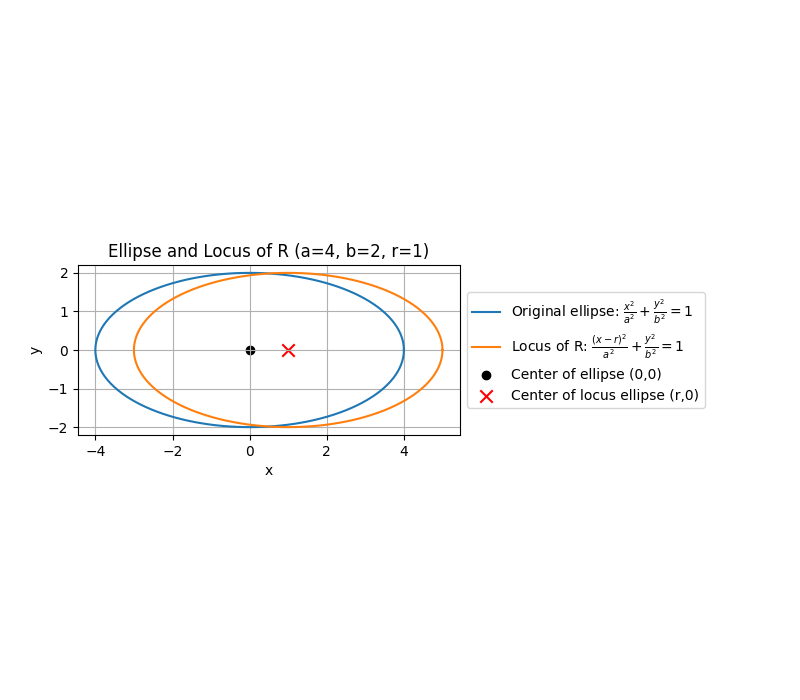
\includegraphics[width=0.5\columnwidth]{figs/1.png}
        \caption{Figure for 8.4.40 for $a=4, b=2, r=1$}
        \label{fig:placeholder}
    \end{figure}
\end{frame}

\end{document}